\documentclass{article}
\usepackage{graphicx} % new way of doing eps files
\usepackage{listings} % nice code layout
\usepackage[usenames]{color} % color
\usepackage{float}
\definecolor{listinggray}{gray}{0.9}
\definecolor{graphgray}{gray}{0.7}
\definecolor{ans}{rgb}{1,0,0}
\definecolor{blue}{rgb}{0,0,1}
% \Verilog{title}{label}{file}
\newcommand{\Verilog}[3]{
  \lstset{language=Verilog}
  \lstset{backgroundcolor=\color{listinggray},rulecolor=\color{blue}}
  \lstset{linewidth=\textwidth}
  \lstset{commentstyle=\textit, stringstyle=\upshape,showspaces=false}
  \lstset{frame=tb}
  \lstinputlisting[caption={#1},label={#2}]{#3}
}


\author{Justin Roessler and Jon Johnston}
\title{Lab 5: Control and Sign Extender}

\begin{document}
\maketitle

\section{Executive Summary}
The purpose of this lab was to make a Control module and a Sign Extender
module for the Decode stage of our proccessor. The Sign Extender module reads in an instruction and extracts the opcode from it. It compares the given opcode to each case of the casex statement (CB, B, LDUR, and STUR). If the opcode does not match any of the cases, it is an R-type and will not be sign extended. When the opcode matches a particular case, it extracts the MSB of its address field and uses that bit to extend the address field to 64 bits.

The Control module works similar to the Sign Extender module, but inside the casex statement it sets the values on all the control wires depending on the opcode. The Control module will test for all 8 commands the proccessor will be able to execute, instead of the Sign Extender only testing 4, and set their cooresponding control wires. After comparing the Expected Results Table and each module's simulation, the lab was successful.	

\section{Test Report}
To verify operation of these modules, this lab requires 2 test benches.
\begin{enumerate}
	\item Control Test Bench
	\item Sign\_Extender Test Bench
\end{enumerate}

% This section should display the Expected Results Table and the Simulation Results for each test bench.  Make sure to label each figure correctly.  Please put them in the order of ERT1, SimResults1, ERT2, SimResults2 so that I can easily compare the ERT and Simulation Results.  To force the figures to be positioned correctly, add the float package (at the top of this file) and use the [H] after {figure} as I did below.  Also, if the ERT is on one page and the Simulation Results are on the next page, you can use a pagebreak as I did below so that the ERT goes to the next page also.

\pagebreak

\begin{figure}[H]
	\begin{center}
		\caption{Expected Results of the Lab 5.}\label{fig:ert_Lab5}
		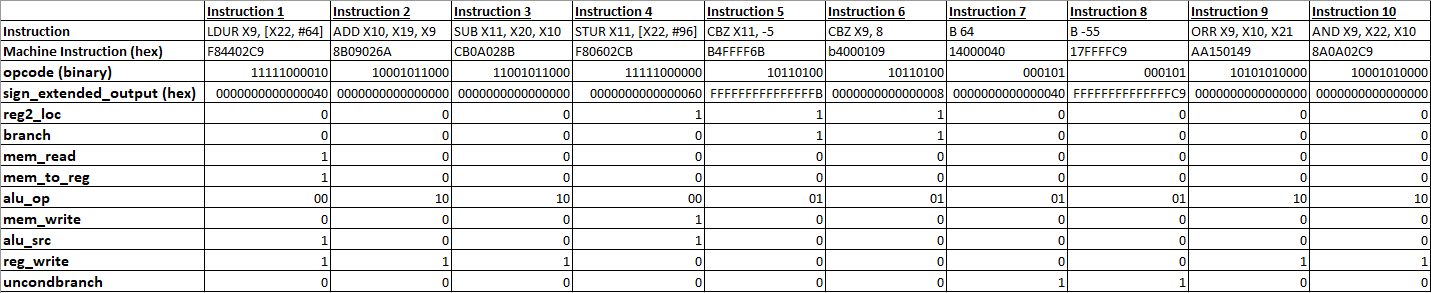
\includegraphics[width=1.0\textwidth]{../images/Lab5Expected.png}
	\end{center}
\end{figure}

\begin{figure}[H]
	\begin{center}
		\caption{Timing diagram for the Control test.}\label{fig:controltest}
		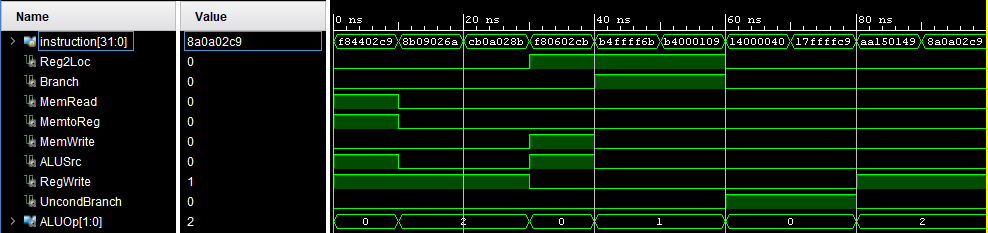
\includegraphics[width=1.0\textwidth]{../images/ControlSimulation.png}
	\end{center}
\end{figure}

\begin{figure}[H]
	\begin{center}
		\caption{Timing diagram for the Sign\_Extender test.}\label{fig:signextendertest}
		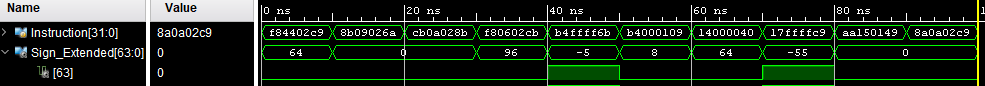
\includegraphics[width=1.0\textwidth]{../images/SignExtenderSimulation.png}
	\end{center}
\end{figure}

\pagebreak
\section{Code Appendix}
% The code appendix should include the test bench code and module code for this lab.
\Verilog{Verilog code for testing the Control Module.}{code:regtest}{../code/2_decode/control_test.v}
\Verilog{Verilog code for implementing the Control Module.}{code:reg}{../code/2_decode/control.v}

\Verilog{Verilog code for testing the Sign\_Extender Module.}{code:regtest}{../code/2_decode/sign_extender_test.v}
\pagebreak
\Verilog{Verilog code for implementing the Sign\_Extender Module.}{code:reg}{../code/2_decode/sign_extender.v}
\end{document} 